% !TeX root = ../main.tex
\chapter{Introduction}

\section{Motivation}

% Motivation - tight resources
A chess engine evaluates a large number of positions during search, and the quality of this evaluation directly affects the strength of the resulting moves. On a desktop system, this evaluation can rely on relatively large neural networks. On a microcontroller, memory, computation, and latency constraints impose tighter limits on the size and cost of the evaluation function. The evaluation function must be small and cheap to run at every node of an alpha-beta search. \emph{Efficiently Updatable Neural Networks} (\textbf{NNUE}) architectures have become a widely used approach for neural evaluation in modern chess engines \parencite{nasu2018}.

\begin{figure}[H]
	\centering
	\includegraphics[width=0.86\textwidth]{../thesis-plots/nnue_incremental_update.png}
	\caption{Incremental update of the NNUE accumulator.}
	\label{fig:nnue-incremental-update-1}
\end{figure}

% bucketing and MoE
A single shallow head must represent positions arising from substantially different tactical and positional regimes. This raises the question of whether different regions of the state space could benefit from specialized heads. Different positions may require understanding of very diverse aspects of the game. Mixture-of-Experts (\textbf{MoE}) evaluation provides a natural framework for this form of specialization \parencite{shazeer2017}: partition the state space into buckets, and assign an \emph{expert head} to each region, while keeping a shared representation. Common chess-engine bucketing strategies rely on manually designed features such as piece count, king location, or game phase \parencite{nasu2018}. Those rules are cheap and interpretable, but they are game-specific heuristics and are not necessarily optimal. They encode what a programmer thinks is a distinct regime, not what the model actually needs in order to specialise.

% Unsupervised alternatives & Literature gap
Unsupervised alternatives exist. Clustering hidden-layer activations groups positions that look similar in the eyes of the network; however, representation similarity does not necessarily reflect similarity in the learning signal. Recent developments in large language models---such as \textbf{ELREA} \parencite{li2025} and \textbf{GradientSpace} \parencite{sridharan2025}---demonstrate that grouping samples by their gradient directions can effectively guide expert specialization. Nevertheless, these techniques target massive LLMs and do not translate directly to embedded environments, where routing overhead and memory footprints are severely restricted. 

This motivates defining partitions via parameter-space directions induced by individual training samples, adapting sample-gradient clustering into a lightweight, data-driven framework suitable for on-device NNUE evaluation without relying on chess-specific heuristics.

\begin{figure}[H]
	\centering
	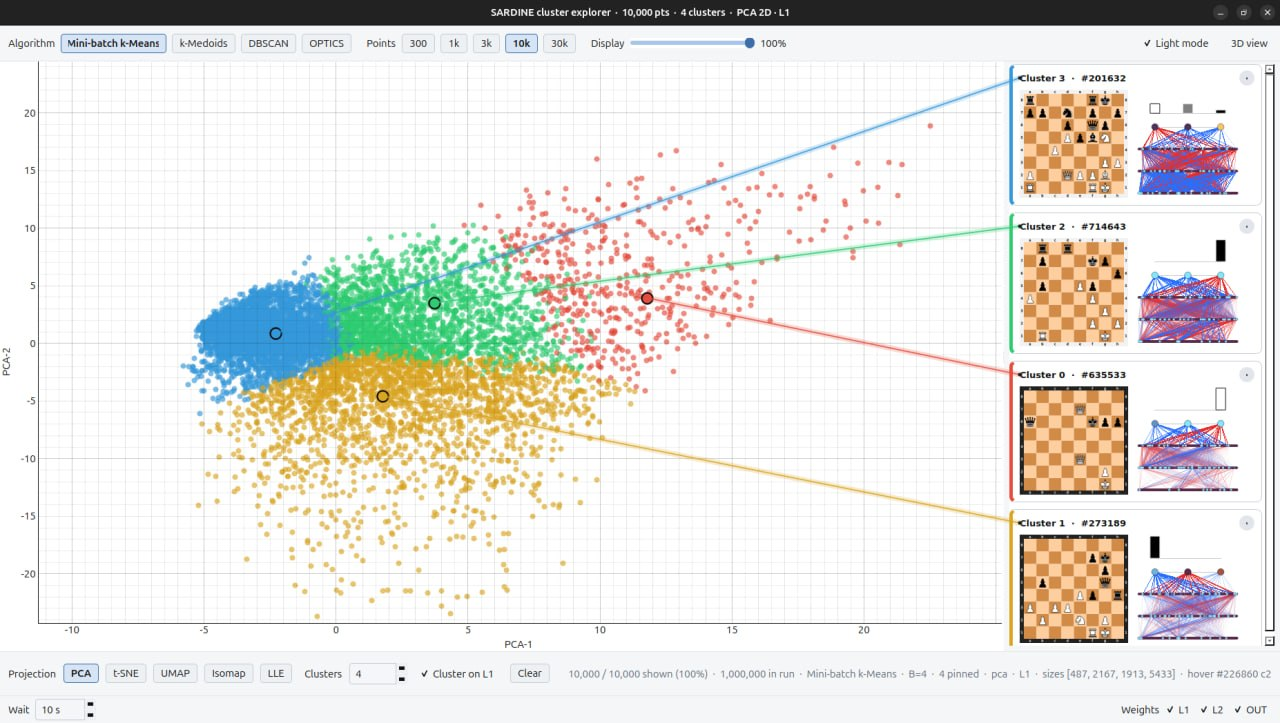
\includegraphics[width=0.86\textwidth]{../thesis-plots/L1_clustering.jpg}
	\caption{Positions clustered by L1 activations and projected to two dimensions.}
	\label{fig:l1-clustering-2}
\end{figure}

\section{Scope of the Thesis}

The central problem addressed in this thesis is the investigation of data-driven approaches for improving neural chess evaluation under the tight memory and computational constraints of embedded devices. In particular, this work explores how the NNUE architecture can be extended to represent different forms of specialization, while retaining the extreme latency efficiency demanded by deep alpha-beta search.

This research investigates how advanced machine learning techniques can be synthesized to enhance neural evaluation. Specifically, we evaluate replacing the standard NNUE accumulator with a learned world-model encoder, compare handcrafted bucketing against unsupervised clustering based on L1 activations and sample gradients, and contrast end-to-end Mixture-of-Experts routing with the Hard MoE paradigm.

These approaches are evaluated from both a learning and deployment perspective. The overarching research question is whether ideas from diverse machine learning paradigms can offer favorable trade-offs between specialization, evaluation quality, and execution efficiency on resource-constrained hardware.

\section{Contributions}

The main contributions of this thesis are summarized as follows:

\begin{itemize}
	\item \textbf{Data-driven State-space Partitioning:} We adapt sample-gradient clustering to NNUE evaluation, creating an unsupervised state-space bucketing scheme that avoids reliance on domain-specific heuristics.
	\item \textbf{Lightweight Routing Mechanism:} We introduce a two-phase architecture where computationally expensive gradient clustering is restricted to offline training, while a lightweight dispatcher predicts expert assignment from frozen accumulator activations during inference.
	\item \textbf{World-Model Integration:} We demonstrate the feasibility of replacing traditional hand-crafted accumulators with a learned world-model encoder, assessing its impact on representation learning and training efficiency.
	%% \item \textbf{Embedded Benchmarking and Deployment:} We quantize and integrate the proposed models into the \emph{Cfish} engine, providing an empirical trade-off analysis between evaluation strength, memory footprint, and search speed on microcontroller hardware.
	\item \textbf{Embedded Benchmarking and Deployment:} We design a quantized integration path for the proposed models in the Cfish engine, specifying the memory layout, integer arithmetic, and inference procedure required for deployment on microcontroller hardware. The empirical analysis of evaluation strength, memory footprint, and search speed is left to future work.
\end{itemize}

\section{Thesis Outline}

The remainder of this thesis is organized as follows:

\begin{itemize}
	\item \textbf{Chapter 2 (Background and Related Work):} Reviews the fundamentals of chess evaluation functions, NNUE architectures, Mixture-of-Experts, and existing sample-gradient specialization techniques.
	\item \textbf{Chapter 3 (Methodology and Experimental Pipeline):} Details the proposed unsupervised bucketing algorithms, sample-gradient clustering, the world-model encoder architecture, and the lightweight routing mechanism.
	\item \textbf{Chapter 4 (Implementation):} Describes the dataset generation, network training, model quantization, and integration with the Cfish engine on embedded hardware.
	\item \textbf{Chapter 5 (Experimental Results):} Presents empirical evaluations regarding expert specialization, evaluation quality, and latency trade-offs compared to single-head and heuristic baselines.
	\item \textbf{Chapter 6 (Discussion):} Interprets the empirical findings, analyzes the routing bottlenecks, and discusses the limitations and generalization of the proposed methods.
	\item \textbf{Chapter 7 (Conclusion and Future Work):} Summarizes the primary findings, discusses current limitations, and outlines directions for future research.
\end{itemize}
